\documentclass{article}
\usepackage{graphicx} % Required for inserting images
\usepackage{hyperref}

\title{MASS-ENERGY EQUIVALENCE}
\author{}

\date{\today}




\begin{document}
\maketitle
\section{EE22B171}
NAME : RUDRA PRATAP SINGH
\newline
GITHUB ID : rps2004
\subsection{INTRODUCTION}
\vspace{0.5cm}
\begin{center}
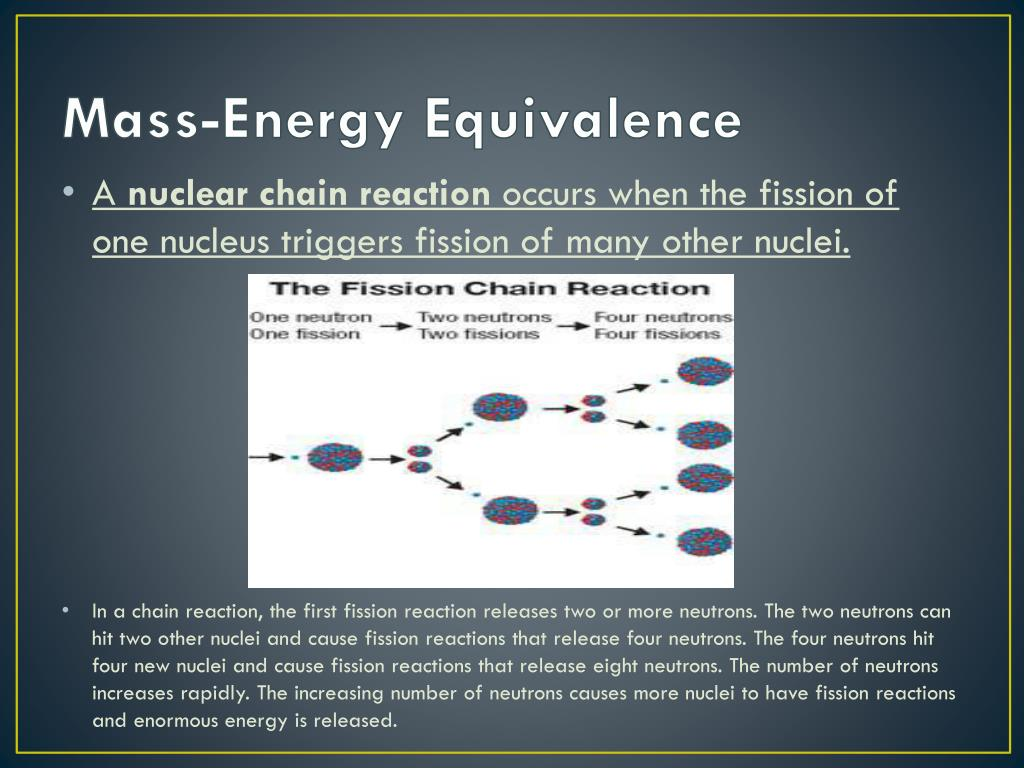
\includegraphics[width=8cm]{mass-energy-equivalence8-l.jpg}
\vspace{2cm}
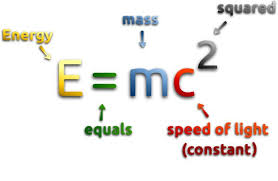
\includegraphics[width=6cm]{energy.jpeg}
\end{center}
\vspace{0.5cm}

Mass–energy equivalence \footnote{\url{https://en.wikipedia.org/wiki/Mass-energy_equivalence}} is the relationship between mass and energy in a system's rest frame, where the two quantities differ only by a multiplicative constant and the units of measurement. The principle is described by the physicist Albert Einstein's formula: 
$E = mc^2$. In a reference frame where the system is moving, its relativistic energy and relativistic mass (instead of rest mass) obey the same formula.
The formula defines the energy E of a particle in its rest frame as the product of mass (m) with the speed of light squared ($c^2$). Because the speed of light is a large number in everyday units (approximately 300000 km/s or 186000 mi/s), the formula implies that a small amount of "rest mass", measured when the system is at rest, corresponds to an enormous amount of energy, which is independent of the composition of the matter.

\subsubsection{Rest Mass}
The mass calculated while the system is at rest is known as Rest mass\footnote{\url{https://en.wikipedia.org/wiki/Mass-energy_equivalence}}, also known as invariant mass. 
It is a physical property that is not dependent on momentum, even when it’s approaching the speed of light at high speeds. 
The invariant mass of Photons, which are massless particles, is zero while free particles, which are massless, consist of energy and momentum. 
The SI units of energy (E) are calculated in joules, mass (m) is calculated in kilograms, and speed of light ‘c’ is calculated in meters per second.

\subsection{Derivation of mass-energy equation}
\subsubsection{Derivation 1}
The simplest method to derive Einstein’s mass-energy equation is as follows\footnote{\url{https:/www.vedantu.com/physics/mass-energy-equivalence}},
Consider an object moving at a speed approximately the speed of light.
A uniform force is acting on it. Due to the applied pressure, energy and momentum are induced in it.
As the force is constant, the increase in momentum of the object= mass x velocity of the body.
We know,
Energy gained= Force x Distance through which force acts

E= F x c 	………………………………………… (1)


Also,


The momentum gained = force x Duration through which force acts


As, momentum = mass x velocity,


The momentum gained = m x c

Hence, Force= m x c ……………………………. (2)


Combining the equation (1) and (2) we get,


$E= mc^2$
\subsubsection{Derivation 2}
Whenever an object is in speed, it seems to get heavier. The following equation\footnote{\url{https:/www.vedantu.com/physics/mass-energy-equivalence}} gives the increase in mass due to speed.

m=$\frac{m_0}{\sqrt{1-\frac{v^2}{c^2}}}$
Where,
m- the mass of the object at the traveling speed

$m_0$- the mass of the object at a stationary position

v- speed of the object

c- speed of the light

We know, in motion, an object possesses kinetic energy and it is given by

E= ½ ($mv^2$)

Total energy possessed by the object is approximately equal to kinetic energy and increases in 
 mass due to speed. 
E = (m$c^2$) + ½ (m$v^2$)


E- (m$c^2$) = ½ (m$v^2)$   , for small $\frac{v}{c}$

E= Relativistic kinetic energy + m$c^2$
The relativistic kinetic energy depends on the kinetic energy and speed of the object. We can simplify the equation by setting the speed of the object as zero. Hence the equations become as follows,
$E= 0+mc^2$
$E= mc^2$
\subsection{Applications}

\begin{itemize}
    \item Einstein's theory was used to understand nuclear fission and fusion reactions. Using the formula, it was revealed that a large amount of energy is liberated during nuclear fission and fusion processes. This phenomenon is used in creating nuclear power and nuclear weapons.
\item  To find out binding energy in an atomic nucleus, the equation is used. By measuring the masses of various nuclei and subtracting them from the sum of masses of protons and neutrons, Binding energy is calculated. Measurement of binding energy is used to calculate the energy released during nuclear reactions. 
\item Einstein’s equation is used to find out the change in mass during the chemical reactions. Whenever there is a chemical reaction, breakage and the formation of new bonds take place. During the exchange of molecules, a change in mass takes place. For chemical energy, Einstein’s equation can be written as


E= $\Delta$m x c2

Where $\Delta$m- change in mass

\end{itemize}



\end{document}
